\documentclass{standalone}
\usepackage{graphicx}	
\usepackage{amssymb, amsmath}
\usepackage{color}

\usepackage{tikz}
\usetikzlibrary{intersections, backgrounds}

\definecolor{light}{RGB}{220, 188, 188}
\definecolor{mid}{RGB}{185, 124, 124}
\definecolor{dark}{RGB}{143, 39, 39}
\definecolor{highlight}{RGB}{180, 31, 180}
\definecolor{gray10}{gray}{0.1}
\definecolor{gray20}{gray}{0.2}
\definecolor{gray30}{gray}{0.3}
\definecolor{gray40}{gray}{0.4}
\definecolor{gray60}{gray}{0.6}
\definecolor{gray70}{gray}{0.7}
\definecolor{gray80}{gray}{0.8}
\definecolor{gray90}{gray}{0.9}
\definecolor{gray95}{gray}{0.95}

\newcommand*{\offset}{0.025}

\begin{document}

\begin{tikzpicture}[scale=0.15, thick] 

  \fill [color=gray90, rounded corners=4pt] (20, -20) rectangle +(20, 60);
  \fill [color=gray90, rounded corners=4pt] (60, -20) rectangle +(20, 60);

  \fill [color=gray90, text=black, line width=1, rounded corners=4pt] (20, 20) rectangle +(20, 20)
  node[midway, align=center] { Hierarchical\\Probability\\Density };
  
  \fill [color=white, text=black, line width=1] (40, 20) rectangle +(20, 20)
  node[midway, align=center] { Individual\\Likelihood\\Function };
  
  \fill [color=gray90, text=black, line width=1, rounded corners=4pt] (60, 20) rectangle +(20, 20)
  node[midway, align=center] { Weakly-Informed\\Posterior\\Density };
  
  \fill [color=white, text=black, line width=1] (80, 20) rectangle +(20, 20)
  node[midway, align=center] { Strongly-Informed\\Posterior\\Density };

  \fill [color=white, text=black, line width=1] (0, 0) rectangle +(20, 20)
  node[midway, align=center] { Centered\\Parameterization };
  
  \filldraw [draw=black, fill=white, line width=1, rounded corners=4pt] (20 + 1, 0 + 1) rectangle +(18, 18);
  \node[] at (30, 10) {
\includegraphics[width=2.5cm]{funnel.eps}};
  
  \filldraw [draw=black, fill=white, line width=1, rounded corners=4pt] (40 + 1, 0 + 1) rectangle +(18, 18);
  \node[] at (50, 10) {
\includegraphics[width=2.5cm]{normal.eps}};
  
  \filldraw [draw=black, fill=white, line width=1, rounded corners=4pt] (60 + 1, 0 + 1) rectangle +(18, 18);
  \node[] at (70, 10) {
\includegraphics[width=2.5cm]{funnel.eps}};
  
  \filldraw [draw=black, fill=white, line width=1, rounded corners=4pt] (80 + 1, 0 + 1) rectangle +(18, 18);
  \node[] at (90, 10) {
\includegraphics[width=2.5cm]{normal.eps}};
  
  \fill [color=white, text=black, line width=1] (0, -20) rectangle +(20, 20)
  node[midway, align=center] { Non-Centered\\Parameterization };
  
  \filldraw [draw=black, fill=white, line width=1, rounded corners=4pt] (20 + 1, -20 + 1) rectangle +(18, 18);
  \node[] at (30, -10) {
\includegraphics[width=2.5cm]{normal.eps}};
  
  \filldraw [draw=black, fill=white, line width=1, rounded corners=4pt] (40 + 1, -20 + 1) rectangle +(18, 18);
  \node[] at (50, -10) {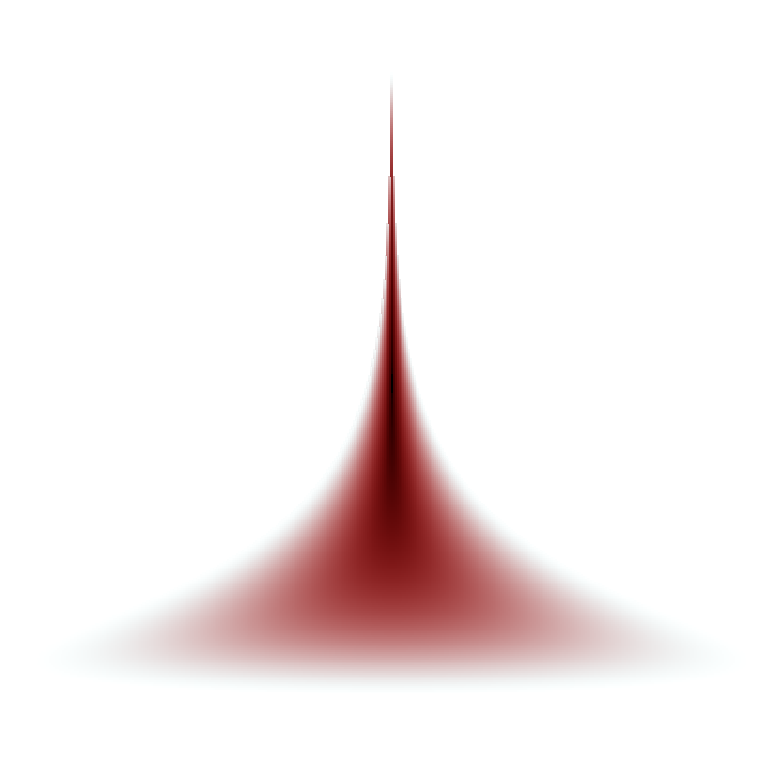
\includegraphics[width=2.5cm]{inverted_funnel.eps}};
  
  \filldraw [draw=black, fill=white, line width=1, rounded corners=4pt] (60 + 1, -20 + 1) rectangle +(18, 18);
  \node[] at (70, -10) {
\includegraphics[width=2.5cm]{normal.eps}};
  
  \filldraw [draw=black, fill=white, line width=1, rounded corners=4pt] (80 + 1, -20 + 1) rectangle +(18, 18);
  \node[] at (90, -10) {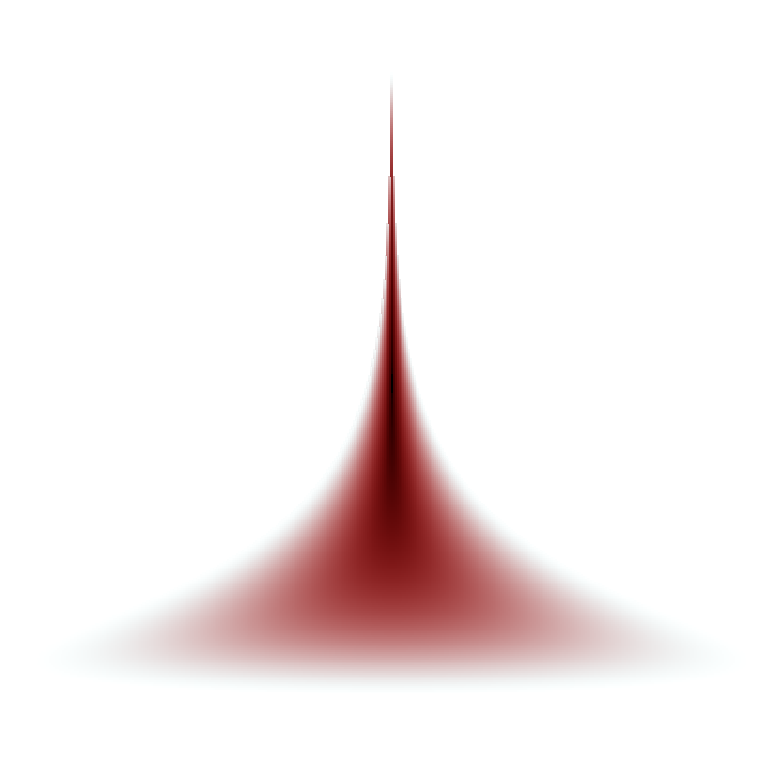
\includegraphics[width=2.5cm]{inverted_funnel.eps}};

\end{tikzpicture}

\end{document}   